\documentclass[a4paper, 12pt]{article}

% ~~~~~~~~~~~~~~~~~~~~~~~~~~~~~~~~~~~~~~~~
% ~~~~~~~~~~~~~~~ PACKAGES ~~~~~~~~~~~~~~~
% ~~~~~~~~~~~~~~~~~~~~~~~~~~~~~~~~~~~~~~~~

\usepackage{amsmath}
\usepackage{relsize}
\usepackage{tikz}
\usepackage{xcolor}
\usetikzlibrary{arrows}
\usetikzlibrary{positioning}

% ~~~~~~~~~~~~~~~~~~~~~~~~~~~~~~~~~~~~~~~~
% ~~~~~~~~~~~~~~~ PREAMBLE ~~~~~~~~~~~~~~~
% ~~~~~~~~~~~~~~~~~~~~~~~~~~~~~~~~~~~~~~~~

\title{Demo Document No. 1\\[0.4em]\smaller{for the SEPTeX module}}
\author{Marcel Simader}
\date{}
\pagenumbering{gobble}
% This is indeed a comment in the preamble

% ~~~~~~~~~~~~~~~~~~~~~~~~~~~~~~~~~~~~
% ~~~~~~~~~~~~~~~ BODY ~~~~~~~~~~~~~~~
% ~~~~~~~~~~~~~~~~~~~~~~~~~~~~~~~~~~~~

\begin{document}
	\maketitle
	
	\noindent This is some text, and it contains a potentially % confusing comment for the "soft" line 
		% wrap % functionality
	
	And this is some text that goes on and on and on and on and on and on and on and on and on and on 
		and on and on and on and on and on and on and on and on and on and on and on\ldots
	This is a \LaTeX\ sentence -- wow!
	\begin{gather*}
		\left[ 1, \frac{1}{3}, 3, \text{abc} \right]
		\left\{ 1, abc, -\frac{3}{5}, -\frac{2}{7} \right\}
		\\
		\left( \left\{ 1, 2, 3, -\frac{9}{2} \right\}, \text{add} \right)
		\left( \left\{ 1, 2, 3, -\frac{9}{2} \right\}, \text{add}, \text{multiply} \right)
	\end{gather*}
	
	\newpage
	
	\begin{figure}[h!]
		\begin{center}
			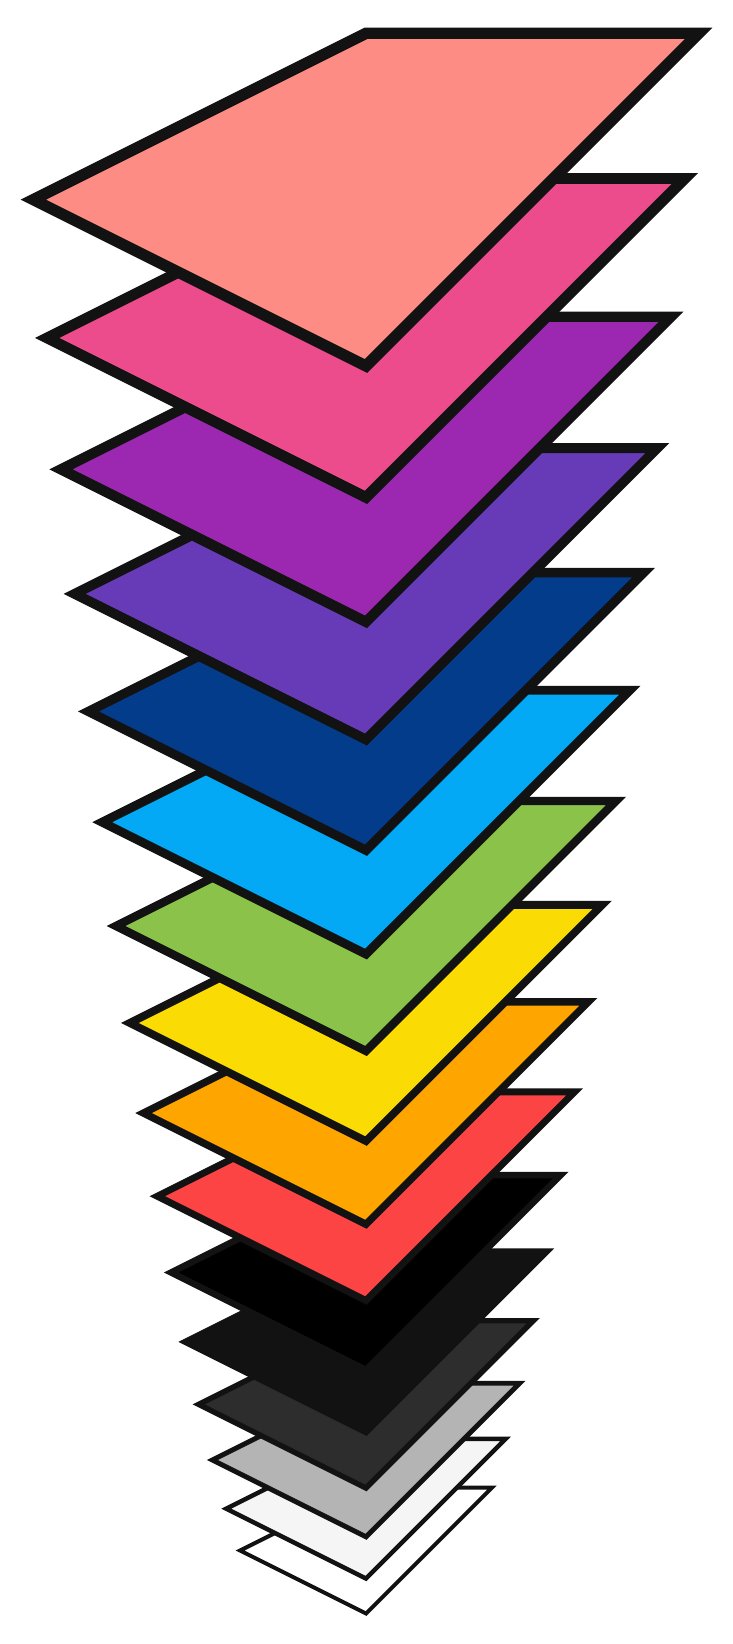
\begin{tikzpicture}[draw]
				\definecolor{WHITE}{RGB}{255, 255, 255}
				\definecolor{ALMOST_WHITE}{RGB}{245, 245, 245}
				\definecolor{LIGHT_GRAY}{RGB}{180, 180, 180}
				\definecolor{DARK_GRAY}{RGB}{45, 45, 45}
				\definecolor{ALMOST_BLACK}{RGB}{18, 18, 18}
				\definecolor{BLACK}{RGB}{0, 0, 0}
				\definecolor{RED}{RGB}{252, 68, 68}
				\definecolor{ORANGE}{RGB}{255, 165, 0}
				\definecolor{YELLOW}{RGB}{251, 219, 4}
				\definecolor{GREEN}{RGB}{139, 195, 74}
				\definecolor{LIGHT_BLUE}{RGB}{3, 169, 244}
				\definecolor{DARK_BLUE}{RGB}{4, 60, 140}
				\definecolor{PURPLE}{RGB}{103, 58, 183}
				\definecolor{MAGENTA}{RGB}{156, 39, 176}
				\definecolor{PINK}{RGB}{236, 76, 140}
				\definecolor{ROSE}{RGB}{252, 140, 132}
				\begin{scope}[draw, scale={0.4}]
					\draw[draw, line width={0.5mm}, color={ALMOST_BLACK!100}, fill={WHITE!100}] ( 0.000, 
						0.000) -- ( 4.000,  4.000) -- ( 0.000,  4.000) -- (-4.000,  2.000) -- cycle;
				\end{scope}
				
				\begin{scope}[draw, scale={0.44375000000000003}]
					\draw[draw, line width={0.5625mm}, color={ALMOST_BLACK!100}, fill={ALMOST_WHITE!100}] 
						( 0.000,  1.000) -- ( 4.000,  5.000) -- ( 0.000,  5.000) -- (-4.000,  3.000) 
						-- cycle;
				\end{scope}
				
				\begin{scope}[draw, scale={0.48750000000000004}]
					\draw[draw, line width={0.625mm}, color={ALMOST_BLACK!100}, fill={LIGHT_GRAY!100}] 
						( 0.000,  2.000) -- ( 4.000,  6.000) -- ( 0.000,  6.000) -- (-4.000,  4.000) 
						-- cycle;
				\end{scope}
				
				\begin{scope}[draw, scale={0.53125}]
					\draw[draw, line width={0.6875mm}, color={ALMOST_BLACK!100}, fill={DARK_GRAY!100}] 
						( 0.000,  3.000) -- ( 4.000,  7.000) -- ( 0.000,  7.000) -- (-4.000,  5.000) 
						-- cycle;
				\end{scope}
				
				\begin{scope}[draw, scale={0.575}]
					\draw[draw, line width={0.75mm}, color={ALMOST_BLACK!100}, fill={ALMOST_BLACK!100}] 
						( 0.000,  4.000) -- ( 4.000,  8.000) -- ( 0.000,  8.000) -- (-4.000,  6.000) 
						-- cycle;
				\end{scope}
				
				\begin{scope}[draw, scale={0.61875}]
					\draw[draw, line width={0.8125mm}, color={ALMOST_BLACK!100}, fill={BLACK!100}] ( 
						0.000,  5.000) -- ( 4.000,  9.000) -- ( 0.000,  9.000) -- (-4.000,  7.000) -- 
						cycle;
				\end{scope}
				
				\begin{scope}[draw, scale={0.6625}]
					\draw[draw, line width={0.875mm}, color={ALMOST_BLACK!100}, fill={RED!100}] ( 0.000, 
						6.000) -- ( 4.000,  10.000) -- ( 0.000,  10.000) -- (-4.000,  8.000) -- cycle;
				\end{scope}
				
				\begin{scope}[draw, scale={0.70625}]
					\draw[draw, line width={0.9375mm}, color={ALMOST_BLACK!100}, fill={ORANGE!100}] ( 
						0.000,  7.000) -- ( 4.000,  11.000) -- ( 0.000,  11.000) -- (-4.000,  9.000) 
						-- cycle;
				\end{scope}
				
				\begin{scope}[draw, scale={0.75}]
					\draw[draw, line width={1.0mm}, color={ALMOST_BLACK!100}, fill={YELLOW!100}] ( 0.000, 
						8.000) -- ( 4.000,  12.000) -- ( 0.000,  12.000) -- (-4.000,  10.000) -- cycle;
				\end{scope}
				
				\begin{scope}[draw, scale={0.79375}]
					\draw[draw, line width={1.0625mm}, color={ALMOST_BLACK!100}, fill={GREEN!100}] ( 
						0.000,  9.000) -- ( 4.000,  13.000) -- ( 0.000,  13.000) -- (-4.000,  11.000) 
						-- cycle;
				\end{scope}
				
				\begin{scope}[draw, scale={0.8375}]
					\draw[draw, line width={1.125mm}, color={ALMOST_BLACK!100}, fill={LIGHT_BLUE!100}] 
						( 0.000,  10.000) -- ( 4.000,  14.000) -- ( 0.000,  14.000) -- (-4.000,  12.000) 
						-- cycle;
				\end{scope}
				
				\begin{scope}[draw, scale={0.88125}]
					\draw[draw, line width={1.1875mm}, color={ALMOST_BLACK!100}, fill={DARK_BLUE!100}] 
						( 0.000,  11.000) -- ( 4.000,  15.000) -- ( 0.000,  15.000) -- (-4.000,  13.000) 
						-- cycle;
				\end{scope}
				
				\begin{scope}[draw, scale={0.9249999999999999}]
					\draw[draw, line width={1.25mm}, color={ALMOST_BLACK!100}, fill={PURPLE!100}] ( 0.000, 
						12.000) -- ( 4.000,  16.000) -- ( 0.000,  16.000) -- (-4.000,  14.000) -- cycle;
				\end{scope}
				
				\begin{scope}[draw, scale={0.96875}]
					\draw[draw, line width={1.3125mm}, color={ALMOST_BLACK!100}, fill={MAGENTA!100}] 
						( 0.000,  13.000) -- ( 4.000,  17.000) -- ( 0.000,  17.000) -- (-4.000,  15.000) 
						-- cycle;
				\end{scope}
				
				\begin{scope}[draw, scale={1.0125}]
					\draw[draw, line width={1.375mm}, color={ALMOST_BLACK!100}, fill={PINK!100}] ( 0.000, 
						14.000) -- ( 4.000,  18.000) -- ( 0.000,  18.000) -- (-4.000,  16.000) -- cycle;
				\end{scope}
				
				\begin{scope}[draw, scale={1.05625}]
					\draw[draw, line width={1.4375mm}, color={ALMOST_BLACK!100}, fill={ROSE!100}] ( 0.000, 
						15.000) -- ( 4.000,  19.000) -- ( 0.000,  19.000) -- (-4.000,  17.000) -- cycle;
				\end{scope}
				
			\end{tikzpicture}
			
		\end{center}
		
		\caption{Captions, Figures, and the Default Colors.}
	\end{figure}
	
	\newpage
	
	\begin{figure}[h!]
		\begin{center}
			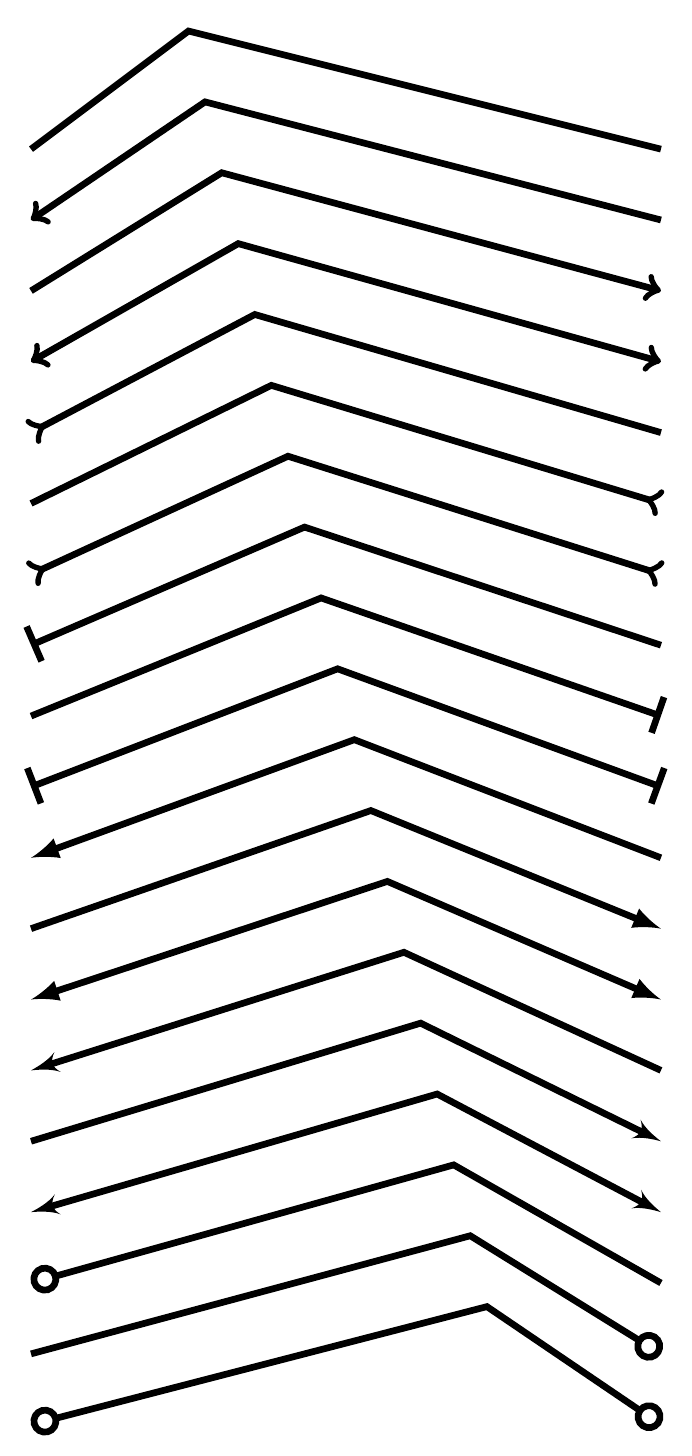
\begin{tikzpicture}[draw]
				\begin{scope}[draw, scale={2}, shift={(0, 0.0)}]
					\draw[-, draw, line width={0.85mm}] ( 0.000,  0.000) to ( 1.000,  0.750) to ( 4.000, 
						0.000);
				\end{scope}
				
				\begin{scope}[draw, scale={2}, shift={(0, -0.45)}]
					\draw[<-, draw, line width={0.85mm}] ( 0.000,  0.000) to ( 1.105,  0.750) to ( 4.000, 
						0.000);
				\end{scope}
				
				\begin{scope}[draw, scale={2}, shift={(0, -0.9)}]
					\draw[->, draw, line width={0.85mm}] ( 0.000,  0.000) to ( 1.211,  0.750) to ( 4.000, 
						0.000);
				\end{scope}
				
				\begin{scope}[draw, scale={2}, shift={(0, -1.35)}]
					\draw[<->, draw, line width={0.85mm}] ( 0.000,  0.000) to ( 1.316,  0.750) to ( 4.000, 
						0.000);
				\end{scope}
				
				\begin{scope}[draw, scale={2}, shift={(0, -1.8)}]
					\draw[>-, draw, line width={0.85mm}] ( 0.000,  0.000) to ( 1.421,  0.750) to ( 4.000, 
						0.000);
				\end{scope}
				
				\begin{scope}[draw, scale={2}, shift={(0, -2.25)}]
					\draw[-<, draw, line width={0.85mm}] ( 0.000,  0.000) to ( 1.526,  0.750) to ( 4.000, 
						0.000);
				\end{scope}
				
				\begin{scope}[draw, scale={2}, shift={(0, -2.7)}]
					\draw[>-<, draw, line width={0.85mm}] ( 0.000,  0.000) to ( 1.632,  0.750) to ( 4.000, 
						0.000);
				\end{scope}
				
				\begin{scope}[draw, scale={2}, shift={(0, -3.15)}]
					\draw[|-, draw, line width={0.85mm}] ( 0.000,  0.000) to ( 1.737,  0.750) to ( 4.000, 
						0.000);
				\end{scope}
				
				\begin{scope}[draw, scale={2}, shift={(0, -3.6)}]
					\draw[-|, draw, line width={0.85mm}] ( 0.000,  0.000) to ( 1.842,  0.750) to ( 4.000, 
						0.000);
				\end{scope}
				
				\begin{scope}[draw, scale={2}, shift={(0, -4.05)}]
					\draw[|-|, draw, line width={0.85mm}] ( 0.000,  0.000) to ( 1.947,  0.750) to ( 4.000, 
						0.000);
				\end{scope}
				
				\begin{scope}[draw, scale={2}, shift={(0, -4.5)}]
					\draw[latex-, draw, line width={0.85mm}] ( 0.000,  0.000) to ( 2.053,  0.750) to 
						( 4.000,  0.000);
				\end{scope}
				
				\begin{scope}[draw, scale={2}, shift={(0, -4.95)}]
					\draw[-latex, draw, line width={0.85mm}] ( 0.000,  0.000) to ( 2.158,  0.750) to 
						( 4.000,  0.000);
				\end{scope}
				
				\begin{scope}[draw, scale={2}, shift={(0, -5.4)}]
					\draw[latex-latex, draw, line width={0.85mm}] ( 0.000,  0.000) to ( 2.263,  0.750) 
						to ( 4.000,  0.000);
				\end{scope}
				
				\begin{scope}[draw, scale={2}, shift={(0, -5.8500000000000005)}]
					\draw[latex'-, draw, line width={0.85mm}] ( 0.000,  0.000) to ( 2.368,  0.750) to 
						( 4.000,  0.000);
				\end{scope}
				
				\begin{scope}[draw, scale={2}, shift={(0, -6.3)}]
					\draw[-latex', draw, line width={0.85mm}] ( 0.000,  0.000) to ( 2.474,  0.750) to 
						( 4.000,  0.000);
				\end{scope}
				
				\begin{scope}[draw, scale={2}, shift={(0, -6.75)}]
					\draw[latex'-latex', draw, line width={0.85mm}] ( 0.000,  0.000) to ( 2.579,  0.750) 
						to ( 4.000,  0.000);
				\end{scope}
				
				\begin{scope}[draw, scale={2}, shift={(0, -7.2)}]
					\draw[o-, draw, line width={0.85mm}] ( 0.000,  0.000) to ( 2.684,  0.750) to ( 4.000, 
						0.000);
				\end{scope}
				
				\begin{scope}[draw, scale={2}, shift={(0, -7.65)}]
					\draw[-o, draw, line width={0.85mm}] ( 0.000,  0.000) to ( 2.789,  0.750) to ( 4.000, 
						0.000);
				\end{scope}
				
				\begin{scope}[draw, scale={2}, shift={(0, -8.1)}]
					\draw[o-o, draw, line width={0.85mm}] ( 0.000,  0.000) to ( 2.895,  0.750) to ( 4.000, 
						0.000);
				\end{scope}
				
			\end{tikzpicture}
			
		\end{center}
		
		\caption{The arrow styles.}
	\end{figure}
	
	\newpage
	
	\begin{figure}[h!]
		\begin{center}
			\begin{tikzpicture}[draw]
				\node[draw, circle] (x11) at (-2.500,  4.330) {11};
				\node[draw, circle] (x0) at ( 0.000,  5.000) {0};
				\node[draw, circle] (x1) at ( 2.500,  4.330) {1};
				\node[draw, circle] (x2) at ( 4.330,  2.500) {2};
				\node[draw, circle] (x3) at ( 5.000,  0.000) {3};
				\node[draw, circle] (x4) at ( 4.330, -2.500) {4};
				\node[draw, circle] (x5) at ( 2.500, -4.330) {5};
				\node[draw, circle] (x6) at ( 0.000, -5.000) {6};
				\node[draw, circle] (x7) at (-2.500, -4.330) {7};
				\node[draw, circle] (x8) at (-4.330, -2.500) {8};
				\node[draw, circle] (x9) at (-5.000, -0.000) {9};
				\node[draw, circle] (x10) at (-4.330,  2.500) {10};
				\draw[-latex', draw, dashed, bend left={15}, line width={0.3mm}] (x11) to (x0);
				\draw[-latex', draw, dashed, bend left={15}, line width={0.3mm}] (x0) to (x1);
				\draw[-latex', draw, dashed, bend left={15}, line width={0.3mm}] (x1) to (x2);
				\draw[-latex', draw, dashed, bend left={15}, line width={0.3mm}] (x2) to (x3);
				\draw[-latex', draw, dashed, bend left={15}, line width={0.3mm}] (x3) to (x4);
				\draw[-latex', draw, dashed, bend left={15}, line width={0.3mm}] (x4) to (x5);
				\draw[-latex', draw, dashed, bend left={15}, line width={0.3mm}] (x5) to (x6);
				\draw[-latex', draw, dashed, bend left={15}, line width={0.3mm}] (x6) to (x7);
				\draw[-latex', draw, dashed, bend left={15}, line width={0.3mm}] (x7) to (x8);
				\draw[-latex', draw, dashed, bend left={15}, line width={0.3mm}] (x8) to (x9);
				\draw[-latex', draw, dashed, bend left={15}, line width={0.3mm}] (x9) to (x10);
				\draw[-latex', draw, dashed, bend left={15}, line width={0.3mm}] (x10) to (x11);
				\draw[-o, draw] (x0) to (x7);
			\end{tikzpicture}
			
		\end{center}
		
		\caption{Nodes, and directed paths -- wow!}
	\end{figure}
	
	\newpage
	
	\begin{figure}[h!]
		\begin{center}
			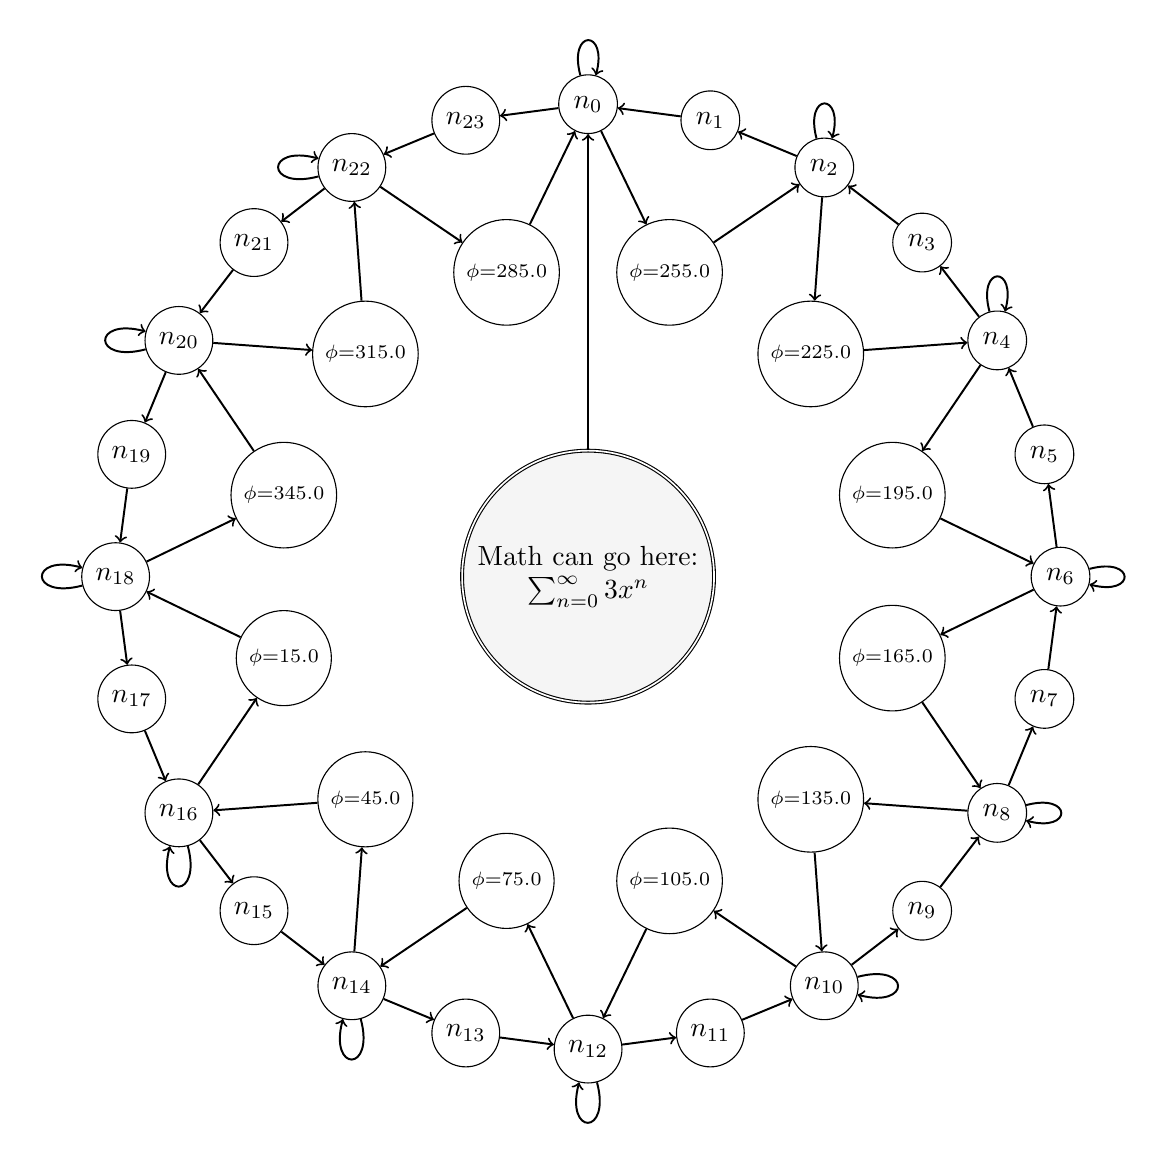
\begin{tikzpicture}[draw]
				\node[draw, circle] (y0) at ( 90.000: 6.000) {$n_{0}$};
				\node[draw, circle] (y1) at ( 75.000: 6.000) {$n_{1}$};
				\node[draw, circle] (y2) at ( 60.000: 6.000) {$n_{2}$};
				\node[draw, circle] (y3) at ( 45.000: 6.000) {$n_{3}$};
				\node[draw, circle] (y4) at ( 30.000: 6.000) {$n_{4}$};
				\node[draw, circle] (y5) at ( 15.000: 6.000) {$n_{5}$};
				\node[draw, circle] (y6) at ( 0.000: 6.000) {$n_{6}$};
				\node[draw, circle] (y7) at ( 345.000: 6.000) {$n_{7}$};
				\node[draw, circle] (y8) at ( 330.000: 6.000) {$n_{8}$};
				\node[draw, circle] (y9) at ( 315.000: 6.000) {$n_{9}$};
				\node[draw, circle] (y10) at ( 300.000: 6.000) {$n_{10}$};
				\node[draw, circle] (y11) at ( 285.000: 6.000) {$n_{11}$};
				\node[draw, circle] (y12) at ( 270.000: 6.000) {$n_{12}$};
				\node[draw, circle] (y13) at ( 255.000: 6.000) {$n_{13}$};
				\node[draw, circle] (y14) at ( 240.000: 6.000) {$n_{14}$};
				\node[draw, circle] (y15) at ( 225.000: 6.000) {$n_{15}$};
				\node[draw, circle] (y16) at ( 210.000: 6.000) {$n_{16}$};
				\node[draw, circle] (y17) at ( 195.000: 6.000) {$n_{17}$};
				\node[draw, circle] (y18) at ( 180.000: 6.000) {$n_{18}$};
				\node[draw, circle] (y19) at ( 165.000: 6.000) {$n_{19}$};
				\node[draw, circle] (y20) at ( 150.000: 6.000) {$n_{20}$};
				\node[draw, circle] (y21) at ( 135.000: 6.000) {$n_{21}$};
				\node[draw, circle] (y22) at ( 120.000: 6.000) {$n_{22}$};
				\node[draw, circle] (y23) at ( 105.000: 6.000) {$n_{23}$};
				\definecolor{ALMOST_WHITE}{RGB}{245, 245, 245}
				\node[draw, circle, double, fill={ALMOST_WHITE!100}, align={center}] (o) at ( 0.000, 
					0.000) {Math can go here: \\$\sum_{n=0}^{\infty} 3x^n$};
				\node[draw, circle] (l1) at ( 1.035,  3.864) {$\scriptstyle \phi = 255.0$};
				\node[draw, circle] (l3) at ( 2.828,  2.828) {$\scriptstyle \phi = 225.0$};
				\node[draw, circle] (l5) at ( 3.864,  1.035) {$\scriptstyle \phi = 195.0$};
				\node[draw, circle] (l7) at ( 3.864, -1.035) {$\scriptstyle \phi = 165.0$};
				\node[draw, circle] (l9) at ( 2.828, -2.828) {$\scriptstyle \phi = 135.0$};
				\node[draw, circle] (l11) at ( 1.035, -3.864) {$\scriptstyle \phi = 105.0$};
				\node[draw, circle] (l13) at (-1.035, -3.864) {$\scriptstyle \phi = 75.0$};
				\node[draw, circle] (l15) at (-2.828, -2.828) {$\scriptstyle \phi = 45.0$};
				\node[draw, circle] (l17) at (-3.864, -1.035) {$\scriptstyle \phi = 15.0$};
				\node[draw, circle] (l19) at (-3.864,  1.035) {$\scriptstyle \phi = 345.0$};
				\node[draw, circle] (l21) at (-2.828,  2.828) {$\scriptstyle \phi = 315.0$};
				\node[draw, circle] (l23) at (-1.035,  3.864) {$\scriptstyle \phi = 285.0$};
				\draw[<-, draw, line width={0.25mm}] (y0) to (o);;
				\draw[<-, draw, line width={0.25mm}] (l1) to (y0);;
				\draw[->, draw, line width={0.25mm}] (l1) to (y2);;
				\draw[<-, draw, line width={0.25mm}] (l3) to (y2);;
				\draw[->, draw, line width={0.25mm}] (l3) to (y4);;
				\draw[<-, draw, line width={0.25mm}] (l5) to (y4);;
				\draw[->, draw, line width={0.25mm}] (l5) to (y6);;
				\draw[<-, draw, line width={0.25mm}] (l7) to (y6);;
				\draw[->, draw, line width={0.25mm}] (l7) to (y8);;
				\draw[<-, draw, line width={0.25mm}] (l9) to (y8);;
				\draw[->, draw, line width={0.25mm}] (l9) to (y10);;
				\draw[<-, draw, line width={0.25mm}] (l11) to (y10);;
				\draw[->, draw, line width={0.25mm}] (l11) to (y12);;
				\draw[<-, draw, line width={0.25mm}] (l13) to (y12);;
				\draw[->, draw, line width={0.25mm}] (l13) to (y14);;
				\draw[<-, draw, line width={0.25mm}] (l15) to (y14);;
				\draw[->, draw, line width={0.25mm}] (l15) to (y16);;
				\draw[<-, draw, line width={0.25mm}] (l17) to (y16);;
				\draw[->, draw, line width={0.25mm}] (l17) to (y18);;
				\draw[<-, draw, line width={0.25mm}] (l19) to (y18);;
				\draw[->, draw, line width={0.25mm}] (l19) to (y20);;
				\draw[<-, draw, line width={0.25mm}] (l21) to (y20);;
				\draw[->, draw, line width={0.25mm}] (l21) to (y22);;
				\draw[<-, draw, line width={0.25mm}] (l23) to (y22);;
				\draw[->, draw, line width={0.25mm}] (l23) to (y0);;
				\draw[<-, draw, line width={0.25mm}] (y0) to (y1);;
				\draw[->, draw, loop above, line width={0.25mm}] (y0) to (y0);;
				\draw[<-, draw, line width={0.25mm}] (y1) to (y2);;
				\draw[<-, draw, line width={0.25mm}] (y2) to (y3);;
				\draw[->, draw, loop above, line width={0.25mm}] (y2) to (y2);;
				\draw[<-, draw, line width={0.25mm}] (y3) to (y4);;
				\draw[<-, draw, line width={0.25mm}] (y4) to (y5);;
				\draw[->, draw, loop above, line width={0.25mm}] (y4) to (y4);;
				\draw[<-, draw, line width={0.25mm}] (y5) to (y6);;
				\draw[<-, draw, line width={0.25mm}] (y6) to (y7);;
				\draw[->, draw, loop right, line width={0.25mm}] (y6) to (y6);;
				\draw[<-, draw, line width={0.25mm}] (y7) to (y8);;
				\draw[<-, draw, line width={0.25mm}] (y8) to (y9);;
				\draw[->, draw, loop right, line width={0.25mm}] (y8) to (y8);;
				\draw[<-, draw, line width={0.25mm}] (y9) to (y10);;
				\draw[<-, draw, line width={0.25mm}] (y10) to (y11);;
				\draw[->, draw, loop right, line width={0.25mm}] (y10) to (y10);;
				\draw[<-, draw, line width={0.25mm}] (y11) to (y12);;
				\draw[<-, draw, line width={0.25mm}] (y12) to (y13);;
				\draw[->, draw, loop below, line width={0.25mm}] (y12) to (y12);;
				\draw[<-, draw, line width={0.25mm}] (y13) to (y14);;
				\draw[<-, draw, line width={0.25mm}] (y14) to (y15);;
				\draw[->, draw, loop below, line width={0.25mm}] (y14) to (y14);;
				\draw[<-, draw, line width={0.25mm}] (y15) to (y16);;
				\draw[<-, draw, line width={0.25mm}] (y16) to (y17);;
				\draw[->, draw, loop below, line width={0.25mm}] (y16) to (y16);;
				\draw[<-, draw, line width={0.25mm}] (y17) to (y18);;
				\draw[<-, draw, line width={0.25mm}] (y18) to (y19);;
				\draw[->, draw, loop left, line width={0.25mm}] (y18) to (y18);;
				\draw[<-, draw, line width={0.25mm}] (y19) to (y20);;
				\draw[<-, draw, line width={0.25mm}] (y20) to (y21);;
				\draw[->, draw, loop left, line width={0.25mm}] (y20) to (y20);;
				\draw[<-, draw, line width={0.25mm}] (y21) to (y22);;
				\draw[<-, draw, line width={0.25mm}] (y22) to (y23);;
				\draw[->, draw, loop left, line width={0.25mm}] (y22) to (y22);;
				\draw[<-, draw, line width={0.25mm}] (y23) to (y0);
			\end{tikzpicture}
			
		\end{center}
		
		\caption{Graphs!}
	\end{figure}
	
\end{document}